\chapter{Preliminaries}
%%% Local Variables:
%%% mode: latex
%%% TeX-master: "thesis"
%%% End:




\section{Controller Area Network (CAN)}
\subsection{Basics}
ISO11898 describes the physical data link layer implementation of \acrshort{can}. This specification describes a twisted-wire pair bus with 120$\Omega$ line impedance, and differential signaling at a rate up to 1 Mbit/s. A network is constructed with two or more transceivers on the same bus lines. The network must be terminated with a 120$\Omega$ resistor at each end of the bus, as shown in Figure \ref{fig:can-bus_topology}.


\begin{figure}[h!]
	\centering
	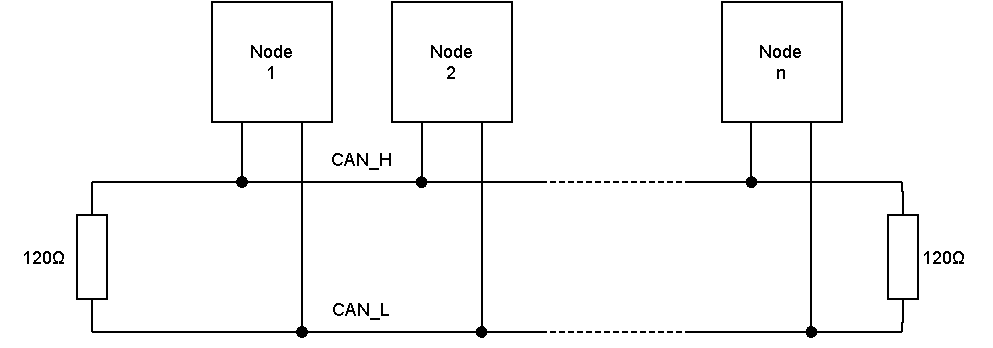
\includegraphics[height=4cm]{images/can-bus_topology}
	\caption{Topology of a \acrshort{can}-Bus}
	\vspace{-1.4ex}
	\label{fig:can-bus_topology}
\end{figure}

As long as the bus is free, any node is allowed to transmit \acrshort{can} messages. Each message is received by all nodes on the network, including the node that sent the message. This type of data broadcasting allows multiple nodes to use the transmitted data. It also allows the sending node to monitor the bus for errors. If two or more nodes try to transmit at the same time, the lower priority message will be overwritten, and this lower priority node will halt transmission upon sensing overwritten bits in its message identifier. The message is then re-transmitted when the bus is again free. This non-destructive process is called bit-wise arbitration.

Every node on the network reads the identifier of a message, and each node independently determines if the message is to be ignored or processed. Since the identifier is specific to the contents of the message rather than the identity of the originating node, new nodes may be added to the network, without modifying the program of any existing node on the network.

\subsection{Frames}
Messages over a CAN Bus are refered to as frames. It compromises of the following parts.

\begin{itemize}
		\item The Arbitration Field, which includes the identifier of the message which also defines the priority of the message. The identifier can contain 11 or 29 bits. 
		\item The data field which contains 0-8 bytes of information
		\item The CRC field which contains a 15-bit checksum. The checksum is used to detect errors in the transmission.
		\item The Acknowledgement Slot, is used to detect if a message was received by any of the devices on the bus. The transmitter checks for the presence of the Acknowledge bit and re-transmits the message if no acknowledge was detected.
		
\end{itemize}

Two different frame formats exist, the standard 
Source: https://www.ti.com/lit/an/slla109a/slla109a.pdf,
https://www.kvaser.com/can-protocol-tutorial/

\section{SAE J1939}
J1939 is the open standard developed by \acrfull{sae}. It is used for networking and communication in the commercial vehicle sector. J1939 is a higher-layer protocol utilizing \acrshort{can} as its physical layer. SAE J1939 is primarily a data driven protocol, providing far better data bandwidth than other automation protocols such as CANopen and DeviceNet. 

The standard specifies CAN bus speeds of 250 kbit/s or 500 kbit/s and uses the extended 29-bit identifier frame format. Most messages defined by the J1939 standard are intended to be broadcast. This means that the data is transmitted on the network without a specific destination. This permits any device to use the data without requiring additional request messages. The 29-bit identifier used in J1939 is structured in the following way.

\begin{figure}[h!]
	\centering
	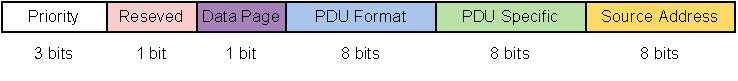
\includegraphics[height=1.5cm]{images/j1939-identifier}
	\caption{29-bit J1939 Identifier}
	\vspace{-1.4ex}
	\label{fig:29-bit_J1939_Identifier}
\end{figure}

The first three bits of the identifier are used for controlling a message priority during the arbitration process. A value of 0 has the highest priority.

The next bit of the identifier is reserved for future use and is set to 0 for transmitted messages.

The next bit in the identifier is the data page selector. This bit expands the number of possible Parameter Groups that can be represented by the identifier.

The PDU format (PF) determines whether the message can be transmitted with a destination address or if the message is always transmitted as a broadcast message.

The interpretation of the PDU specific (PS) field changes based on the PF value:

If the PF is between 0 and 239, the message is addressable (PDU1) and the PS field contains the destination address.
If the PF is between 240 and 255, the message can only be broadcast (PDU2) and the PS field contains a Group Extension.
The Group extension expands the number of possible broadcast Parameter Groups that can be represented by the identifier.

The term Parameter Group Number (PGN) is used to refer to the value of the Reserve bit, DP, PF, and PS fields combined into a single 18 bit value.
\todo{this is just copied in for now, think about if we really need that}

Source: https://copperhilltech.com/a-brief-introduction-to-the-sae-j1939-protocol/,
https://www.kvaser.com/about-can/higher-layer-protocols/j1939-introduction/
\newpage

\section{Fleet Management System (FMS)}
The Fleet Management Systems Interface (FMS) is a standard interface developed by European commercial vehicle manufacturers in 2002. It defines a common interface for telematics applications and include driving as well as diagnostics information. The data is coded according to the SAE J1939 standard. FMS is a broadcast only system, a gateway between the internal bus and the FMS bus is implemented by the OEM. 3rd party systems, like the Fleet-Monitor, are forbidden on the internal bus as shown in figure \ref{fig:fms-bus}. 

\begin{figure}[h!]
	\centering
	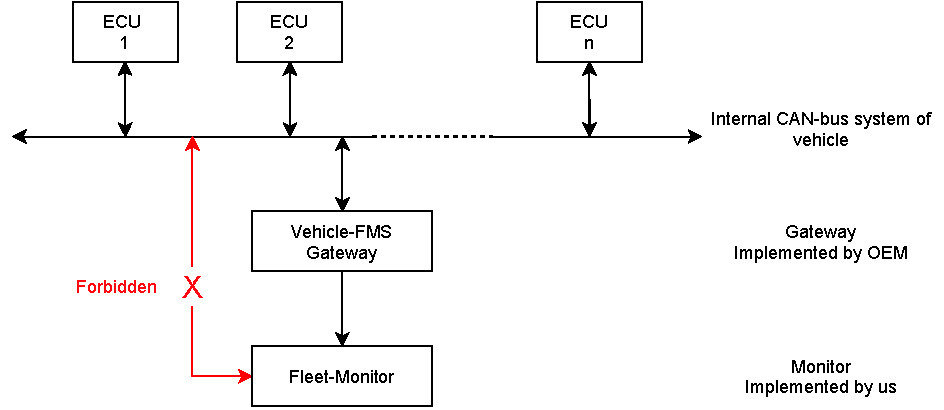
\includegraphics[height=6.5cm]{images/fms-bus}
	\caption{FMS Topology}
	\vspace{-1.4ex}
	\label{fig:fms-bus}
\end{figure}

As of writing the FMS Standard includes 44 different packages. Each frame has a fixed data length of 8 byte which makes decoding a lot easier.   

